\documentclass{article}
\usepackage{bm}
\usepackage{amsmath}
\usepackage{graphicx}
\usepackage{mdwlist}
\usepackage[colorlinks=true]{hyperref}
\usepackage{geometry}
\usepackage{kotex}
\geometry{margin=1in}
\geometry{headheight=2in}
\geometry{top=2in}
\usepackage{palatino}
%\renewcommand{\rmdefault}{palatino}
\usepackage{fancyhdr}
%\pagestyle{fancy}
\rhead{}
\lhead{}
\chead{%
  {\vbox{%
      \vspace{2mm}
      \large
      Hardware System Design 4190.309A\hfill
\\
      Seoul National University
      \\[4mm]
      \textbf{Practice \#4. How to use IP catalog \& Synthesize}\\
      \textbf{Jiwon Lee, Sangjun Son}
    }
  }
}

%%%%%%%%%%%%%%%%%%%%%%%
\usepackage{xcolor}
\usepackage{listings}
\definecolor{vgreen}{RGB}{104,180,104}
\definecolor{vblue}{RGB}{49,49,255}
\definecolor{vorange}{RGB}{255,143,102}

\lstdefinestyle{verilog-style}
{
    language=Verilog,
    basicstyle=\small\ttfamily,
    keywordstyle=\color{vblue},
    identifierstyle=\color{black},
    commentstyle=\color{vgreen},
    numbers=left,
    numberstyle=\tiny\color{black},
    numbersep=10pt,
    tabsize=8,
    moredelim=*[s][\colorIndex]{[}{]},
    literate=*{:}{:}1
}

\makeatletter
\newcommand*\@lbracket{[}
\newcommand*\@rbracket{]}
\newcommand*\@colon{:}
\newcommand*\colorIndex{%
    \edef\@temp{\the\lst@token}%
    \ifx\@temp\@lbracket \color{black}%
    \else\ifx\@temp\@rbracket \color{black}%
    \else\ifx\@temp\@colon \color{black}%
    \else \color{vorange}%
    \fi\fi\fi
}
\makeatother

\usepackage{trace}
%%%%%%%%%%%%%%%%%%%%%%%

\usepackage{paralist}

\usepackage{todonotes}
\setlength{\marginparwidth}{2.15cm}

\usepackage{tikz}
\usetikzlibrary{positioning,shapes,backgrounds}

\begin{document}
\pagestyle{fancy}

\section*{Goal}

\begin{itemize*}
\item Implement base of Float32 multiplier + accumulator.
\item Implement Floating point / Integer fused multiply-adder using IP catalog.
\item Implement adder-array using accumulator module.
\end{itemize*}

\section{Implementation}

\subsection{Floating point fused multiply-adder}

이번 프로젝트는 IP catalog를 이용해보는 과제였기 때문에, 미리 구현된 floating point multiply-adder를 사용하고
testbench 에서 입력값을 조정하여 출력값을 확인하였다.
Verliog의 floating point representation은 IEEE 754 standard를 사용한다. 
즉, 32bit binary number는 다음과 같은 형태로 floating point로 전환된다. 
\begin{equation}
	 f = sign \times 2^{exponent} \times mantissa
\label{eqn1}
\end{equation}

IEEE 754의 부동소수점 표현은 크게 세 부분으로 구성되는데, 최상위 비트는 부호를 표시하는데 사용되며, 지수 부분 (exponent)과 가수 부분 (fraction/mantissa)이 있다.
이를 시각적으로 나타내면 Figure~\ref{fig1} 같다.

\begin{figure}[ht]
	\centering
	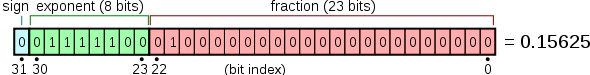
\includegraphics[width=1.0\textwidth]{fig/fig1.png}
	\caption{IEEE 754 single-precision binary floating-point format: binary32}
\label{fig1}
\end{figure}

결과값을 확인하기 위해 sign, exponent 그리고 mantissa 부분의 분포를 uniformly random 하게 만들기 위해서 Equation~\ref{eqn2}와 같은 범위 사이의 숫자를 뽑아 이어붙이는 식으로 입력값을 산정하여 test를 진행하였다.
\begin{equation}
	 sign \in [0, 2^1), \quad exponent \in [0, 2^8), \quad mantissa \in [0, 2^{23})
\label{eqn2}
\end{equation}
\begin{equation}
	 f = (sign \ll 31) + (exponent  \ll 23) + (mantissa)
\label{eqn3}
\end{equation}

위와 같은 방법으로 생성된 테스트 값들은 다음 Table~\ref{tab1}과 같다. 테스트에 사용된 입력값과 더불어 실험 결과값 또한 가시성을 높이기 위해 첨부하였다. IEEE 754의 모든 부분이 uniformly random 하게 선택되기 때문에 nan 또는 inf 값이 나올 수 있으며 해당 값에 따라 연산값이 바뀌는 것을 확인할 수 있다.
\begin{table}[ht]
\renewcommand{\arraystretch}{1.5}
\begin{center}
\begin{tabular}{ |c | ccc | c |} 
 \hline
 $i$ & $a_{in}[31:0]$ & $b_{in}[31:0]$ & $c_{in}[31:0]$ & $res[31:0]$  \\ 
 \hline
1 & $-2.131260 \times 10^{23}$ 		& $4.226937 \times 10^{-22}$		& $-5.057321 \times 10^{-37}$	& $-5.057321 \times 10^{-37}$ \\
2 & $-9.676296 \times 10^{-24}$ 		& $-5.898969 \times 10^{20}$ 		& $-2.102489 \times 10^{14}$	& $-5.057321 \times 10^{-37}$  \\ 
\vdots& & \vdots & & \vdots \\
3 & $-9.676296 \times 10^{-24}$ 		& $-5.898969 \times 10^{20}$ 		& $-2.102489 \times 10^{14}$	& $-5.057321 \times 10^{-37}$  \\ 
 \hline
\end{tabular}
\caption{Your caption.}\label{tab1}
\end{center}
\end{table}



\begin{lstlisting}[style={verilog-style}]
`timescale 1ns / 1ps
module my_add #(
    parameter BITWIDTH = 32
)
(
    input [BITWIDTH-1:0] ain,
    input [BITWIDTH-1:0] bin,
    output [BITWIDTH-1:0] dout,
    output overflow
);
    // concatnate (overflow, dout) & detect overflow
    assign {overflow, dout} = ain + bin;
endmodule
\end{lstlisting}

\section{Results \& Conclusion}

\subsection{Adder}
testbench에서 주어지는 ain, bin의 값은 0 ~ $2^{31}-1$ 까지의 임의의 값이다.
따라서, dout의 값은 최대 $2^{31}-2$  이고, 이는 32bit로 만들 수 있는 최댓값인 $2^{31}-1$  보다 작으므로 주어진 testbench에서는 overflow가 발생하지 않는다.
하지만, 실제로 ain, bin의 값을 증가시켜 overflow가 발생하도록 하였을 때, overflow bit가 1이 되어 detecting한다는 것을 알 수 있었다.


\end{document}
